\section{Attacks' principles}
\subsection{Birthday Paradox}
This Paradox is not an actual one, but is the result of a cognitive bias. \newline
The idea is that in a room full of people, the probability of having no one with matching birthdays is actually lower than expected.\newline
Consider what follows:
\begin{itemize}
    \item Let $n$ be the number of possible birthdays
    \item Let $N$ be the number of people.
    \item Let $S$ be a space $\{1, \dots, n\}^{N} \ni (c_{1}, \dots, c_{N})$.
    \item The probability of a given combination of birthdays to happen is then:
    \[
    \mathbb{P}[(c_{1}, \dots, c_{N})] = n^{-N} = \frac{1}{|S|}
    \]
    \item Let's now compute the probability of having \textbf{no collisions}:
    \begin{align*}
        p(N) &= \mathbb{P}[\forall i \neq j: c_{i} \neq c_{j}] \\
        &= \frac{\prod_{i=0}^{N-1} n - i}{n^{N}} \\
        &= \frac{n \cdot (n-1) \cdot \dots \cdot (n - N + 1)}{n \cdot n \cdot \dots \cdot n} \\
        &= \prod_{i=0}^{N-1} 1 - \frac{i}{n}
    \end{align*}
    \item Let'now compute the probability of having \textbf{at least one collision}:
    \begin{align*}
        q(N) &= 1 - p(N) \geq 1 - \epsilon \\
        & \iff p(N) \leq \epsilon
    \end{align*}
    \item Let's now consider that:
    \begin{align*}
        p(N) = \prod_{i=0}^{N-1} 1 - \frac{i}{n} &\leq \prod_{i=0}^{N-1} e^{-\frac{i}{n}}\\
        & = e^{\sum_{i=0}^{N-1}-\frac{i}{n}}\\
        & = e^{-\frac{1}{n}\sum_{i=0}^{N-1}i}\\
        & = e^{-\frac{(N)(N-1)}{2n}} \leq \epsilon
    \end{align*}
    Therefore,
    \[
        N \geq \frac{1+\sqrt{1 - 8n \operatorname{log}(\epsilon)}}{2} \simeq \sqrt{n |\operatorname{log}(\epsilon)|}
    \]
    \item So, when $N \simeq n$, then $\epsilon \simeq \frac{1}{2}$
\end{itemize}

\section{Attacks to RSA}
\subsection{Chosen-ciphertext/Known-plaintext attack}
This attacks can happen when the attacker knows a portion or the complete plaintext $m$ associated to the ciphertext $c$.\newline
The attacks proceeds as follows:
\begin{itemize}
    \item The attacker $E$ generates a random number $r \in \mathbb{Z}_{n_{A}}^{*}$, so $(r, n_{A}) = 1$. This quantity is called the "blinding factor".
    \item $E$ asks $A$ to sign the quantity
    \[r^{c_{A}} \cdot c \bmod n_{A}\]
    In this way, $r^{c_{A}} \cdot c$ acts like a random message.
    \item If $A$ signs $r^{c_{A}} \cdot c$, it gets:
    \begin{align*}
        f_{A}^{-1}(r^{c_{A}} \cdot c) &= (r^{c_{A}} \cdot c)^{d_{A}} \\
        &= r^{c_{A}d_{A}} \cdot c^{d_{A}} \bmod n_{A} \\
        &= r \cdot m \bmod n_{A}
    \end{align*}
    Since $r \cdot m$ looks random, it's hard to identify the attack here.
    \item Now that $E$ has the quantity $r \cdot m \bmod n_{A}$, and since he produced $r$, he knows $r^{-1} \bmod n_{A}$.\\
    Therefore, he can compute:
    \[r^{-1} \cdot r \cdot m \bmod n_{A} = m\]
\end{itemize}
\begin{figure}[h]
    \centering
    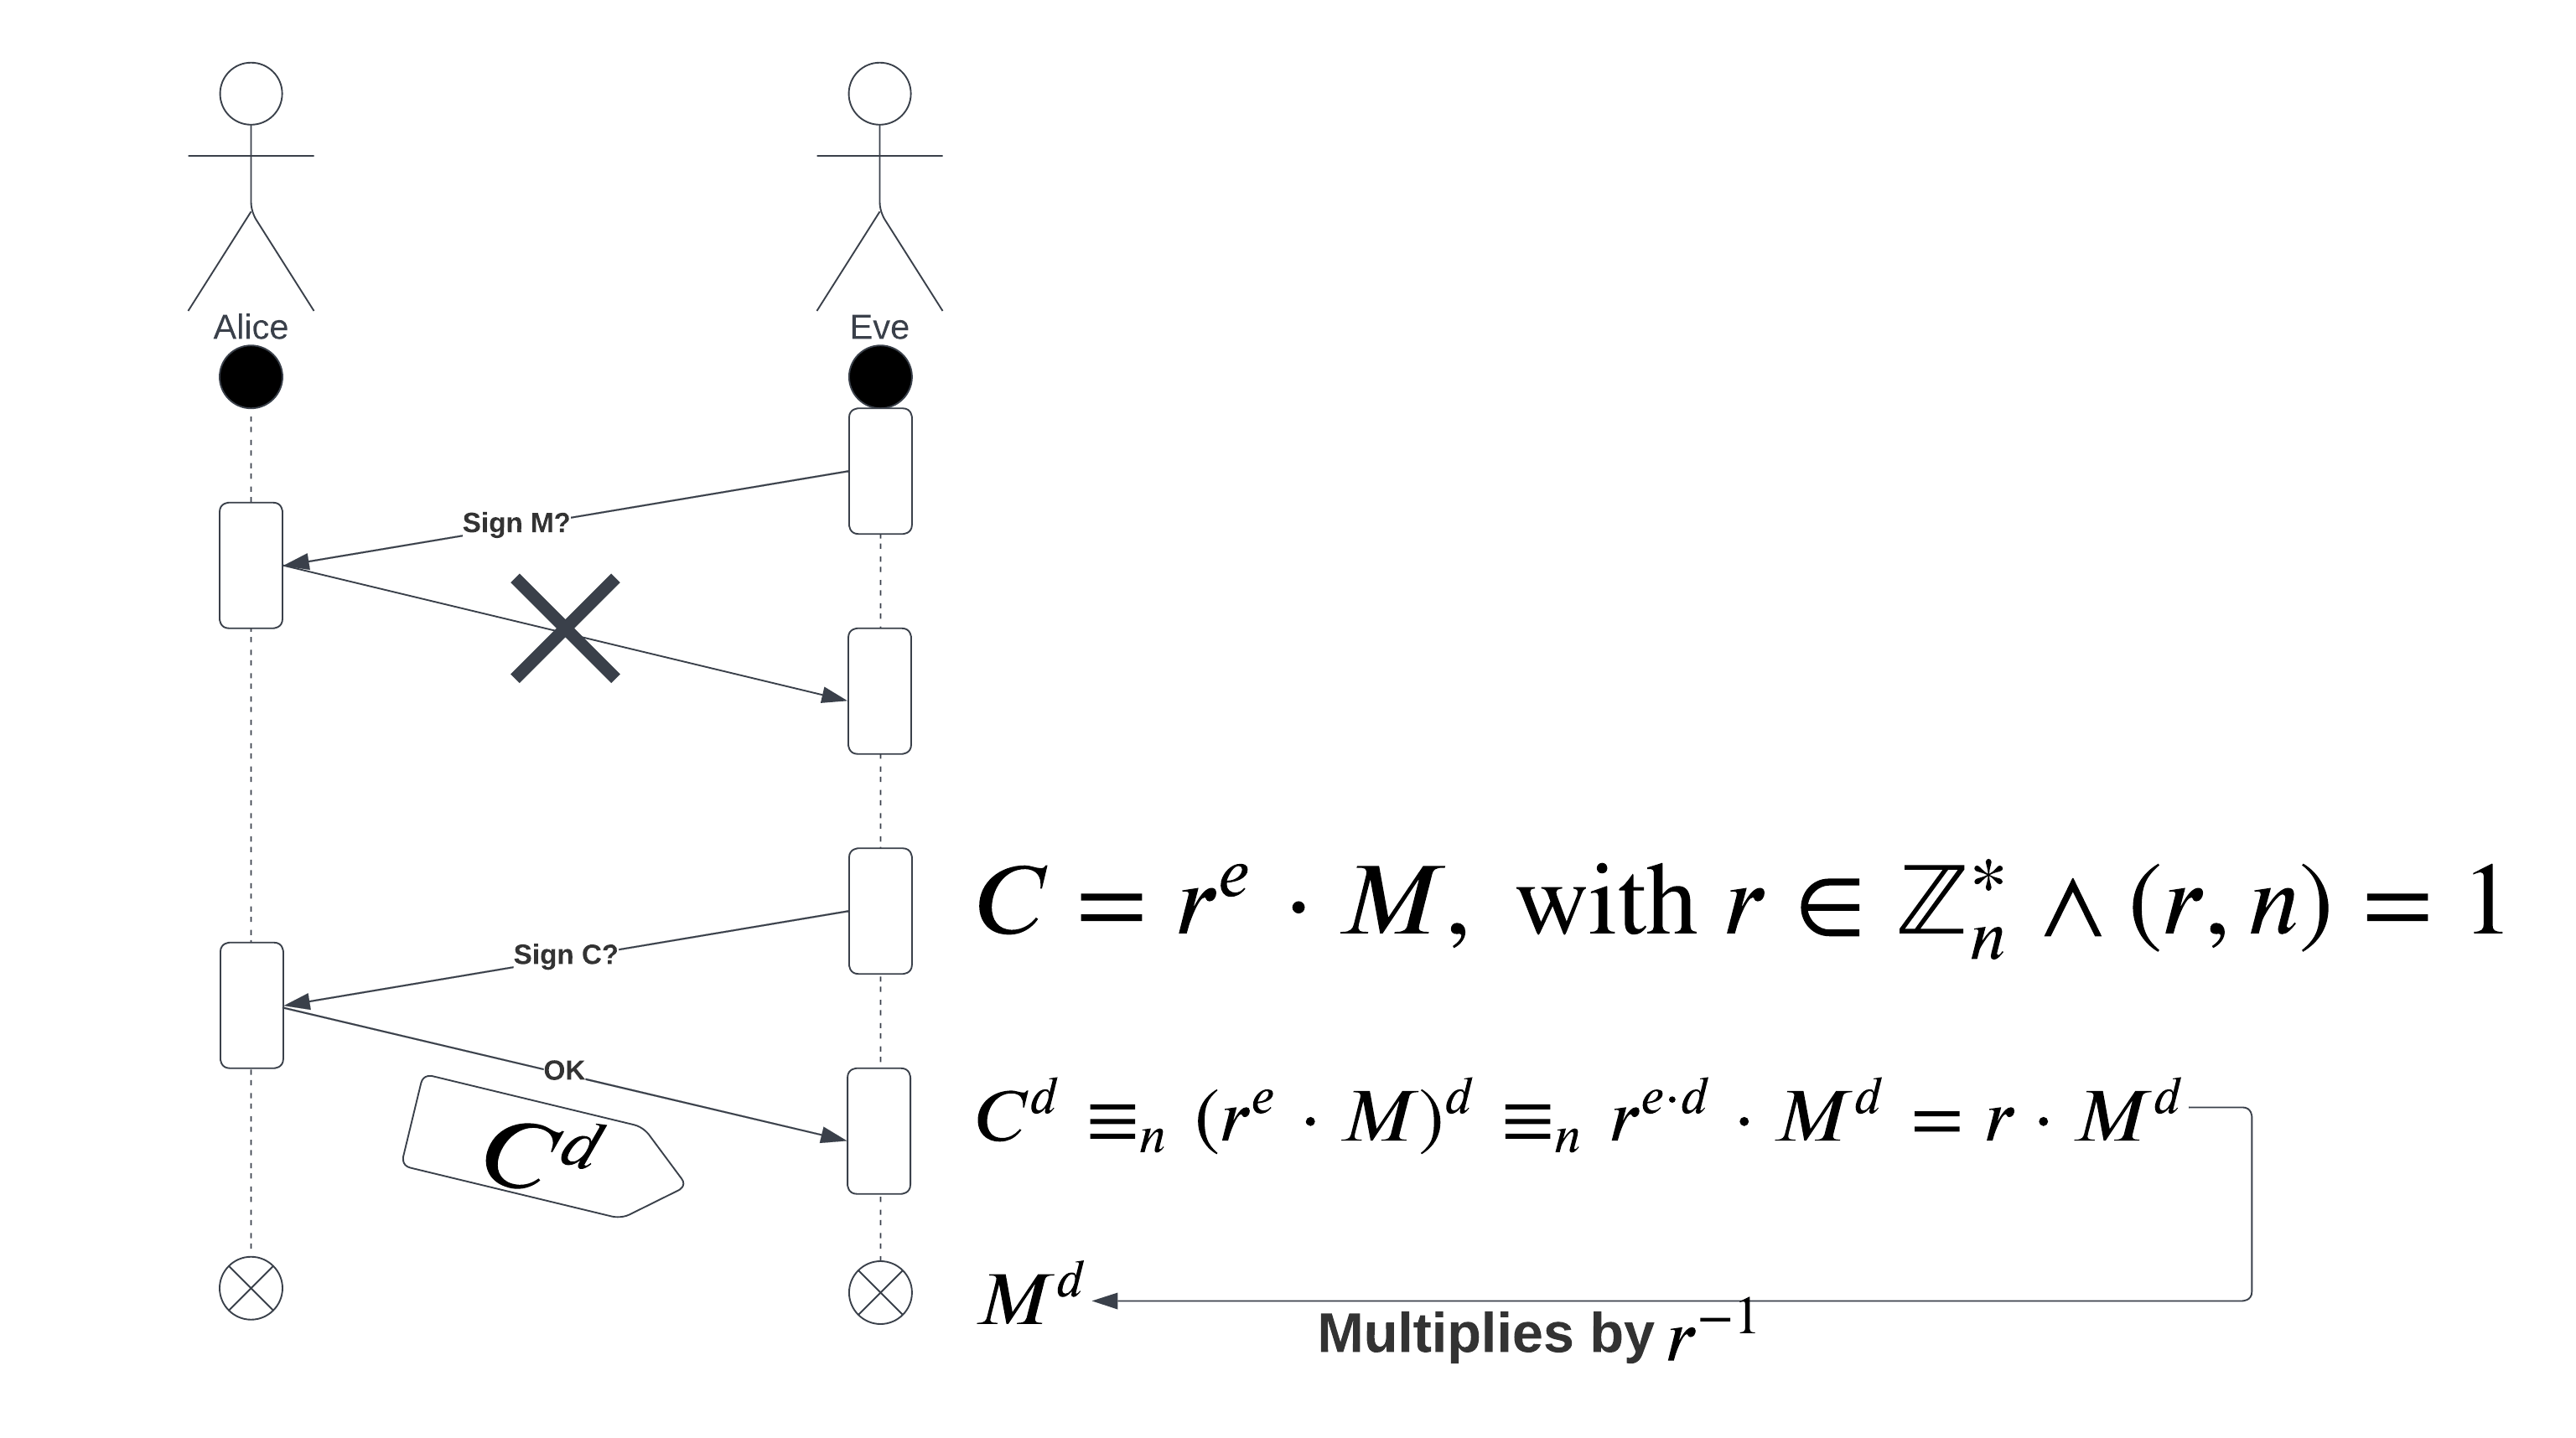
\includegraphics[width=\textwidth]{img/RSA_attack_knownp.png}
    \caption{Attack to Digital Signature that uses RSA cryptosystem.}
\end{figure}

\subsection{Random fault attack}
This attack on RSA can be done when a signature is computed incorrectly. \newline
Recall that the digital signature with RSA works as follows.\newline
Alice computes:
\[s = m^{d} (\bmod n)\]
Bob, to verify the signature, computes:
\[s^{e} = m (\bmod n)\]
Where:
\begin{itemize}
    \item $s$ is the signature;
    \item $m$ is the cleartext message;
    \item $d$ is the private key (exponent);
    \item $n$ is the public key (modulus);
    \item $e$ is the public key (exponent).
\end{itemize}
This attack exploits an optimization that is commonly used to compute the signature. \newline
Since $n$ is the product of two big prime numbers $p, q$, the CRT (Chinese Reminder Theorem) can be used to compute two smaller modulus ($p, q$ respectivly), instead of a bigger one.
\[
     \begin{cases}
       s_{1} \equiv m^{d_{p}} (\bmod p) \\
       s_{2} \equiv m^{d_{q}} (\bmod q)
     \end{cases}
     \Longrightarrow s (\bmod pq)
\]
Consider now the case when $s_{2}$ is uncorrectly computed:
\[
     \begin{cases}
       s_{1} \equiv m^{d_{p}} (\bmod p) \\
       \hat{s_{2}} \equiv m^{d_{q}} (\bmod q)
     \end{cases}
     \Longrightarrow \hat{s} (\bmod pq)
\]
Then we have that:
\[
     \begin{cases}
       s^{e} \equiv m (\bmod p) \\
       \hat{s^{e}} \not\equiv m (\bmod q)
     \end{cases}
     \Longrightarrow
     \begin{cases}
       s^{e} - m \equiv 0 (\bmod p)\\
       \hat{s^{e}} - m \not\equiv 0 (\bmod q)
     \end{cases}
     \Longrightarrow
     \begin{cases}
       p | s^{e} - m\\
       q \nmid \hat{s^{e}} - m
     \end{cases}
\]
Therefore, exists some $k$ such that:
\[p \cdot k = \hat{s^{e}} - m\]
Therefore, we can obtain easily $p$ by computing $gcd(s^{e} - m, N)$.

\subsection{RSA basic attack}
This attack is conducted when Alice sends to Bob1 and Bob2 the same message, by using the same public key (modulus). Assume what follows:
\begin{itemize}
    \item \[n_{X} = n_{Y}\]
    \item \[(e_{X}, e_{Y}) = 1\]
\end{itemize}
Therefore, an intruder can compute $r,s$ such that:
\[r \cdot e_{X} + s \cdot e_{Y} = 1\]
By using the \emph{Extended Euclidean Algorithm} (recall that $e_{X}, e_{Y}$ are public). Since $e_{X}, e_{Y}$ are positive, then one between $r, s$ must be negative. Then:
\begin{itemize}
    \item The intruder computes $c_{1}^{-1} \bmod n_{X}$, using the \emph{E.E.A.}.
    \item The intruder then computes:
    \begin{align*}
        (c_{1}^{-1})^{-r} \cdot c_{2}^{s} & =\\
        (M^{-e_{X}})^{-r} \cdot M^{e_{Y} \cdot s} & =\\
        M^{r \cdot e_{X} + s \cdot e_{Y}} \bmod n_{X} & =\\
        M \bmod n_{X}
    \end{align*}
\end{itemize}
Therefore, if different public keys aren't used, an intruder can easily intercept a broadcasted message.
\begin{figure}[h]
    \centering
    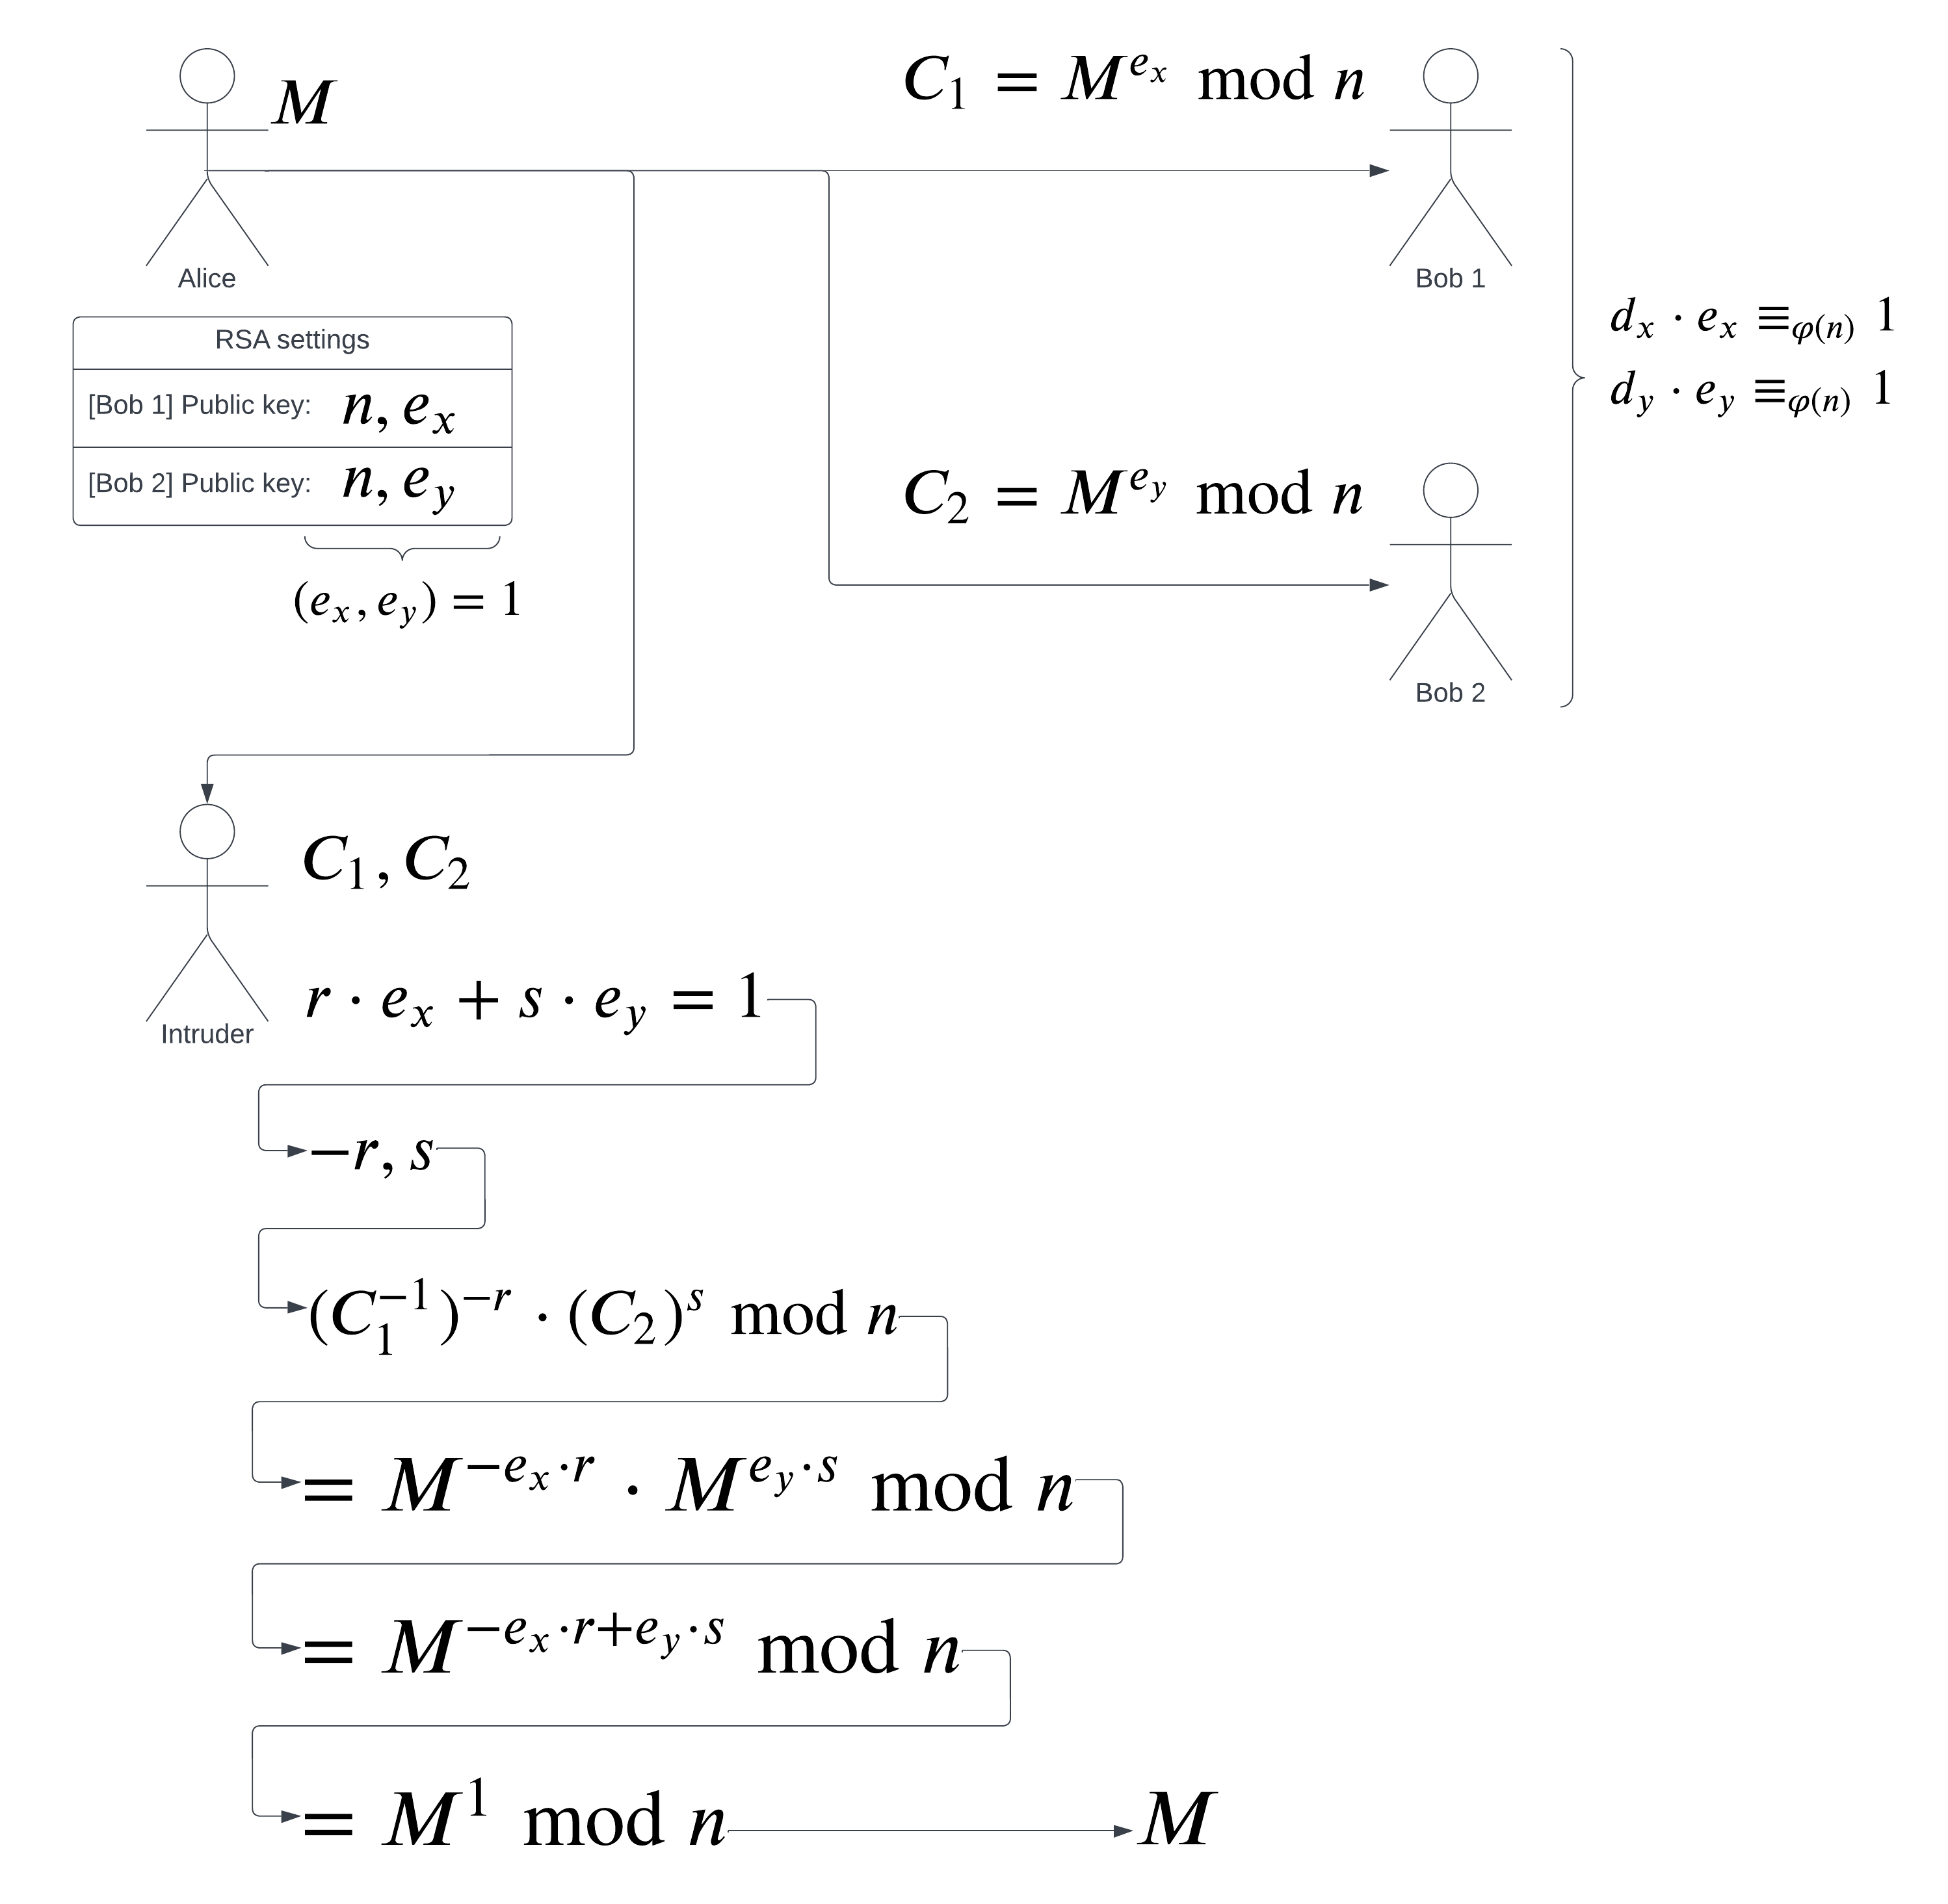
\includegraphics[width=\textwidth]{img/RSA_attack_basic.png}
    \caption{Basic RSA attack on broadcast communication.}
\end{figure}

\subsection{Broadcast attack}
In this attack, the user broadcasts a message by using different values for each receiver ($\forall i \neq j: n_{i} \neq n_{j}$), but uses the same value of $e$ for everyone. We'll assume that $r \geq e$.\newline
The attack is conducted as follows:
\begin{itemize}
    \item The intruder collects $C_{1}, C_{2}, \dots, C_{r}$, the cyhpered texts.
    \item The intruder uses a subset of the cyphered texts $D \subset \{C_{1}, C_{2}, \dots, C_{r}\}$. Consider $|D| = e$.
    \item The intruder solves the system of equations
    \[C \equiv_{n} C_{i}, \forall i = 1, 2, \dots, e\]
    \item $C$ is the unique solution to the system, due to the Chinese Reminder Theorem.
    \item Consider that:
    \begin{align*}
        M \in \mathbb{Z}_{n_{i}}^{*} \forall i = 1, 2, \dots, e \implies &\\
        M < n_{i} \forall i = 1, 2, \dots, e \implies &\\
        M^{2} < n_{1} \cdot n_{2} \implies &\\
        M^{e} < \prod_{i=1}^{e} n_{i} = N \implies &\\
        M^{e} = C \iff M = C^{\frac{1}{e}}
    \end{align*}
    Therefore, finding the solution in modulus $N$ is equivalent to find the solution to the system.
\end{itemize}
In order to prevent this kind of attack, when using RSA in broadcasts is important to use different values for $e,n$ for each user.
\begin{figure}[h]
    \centering
    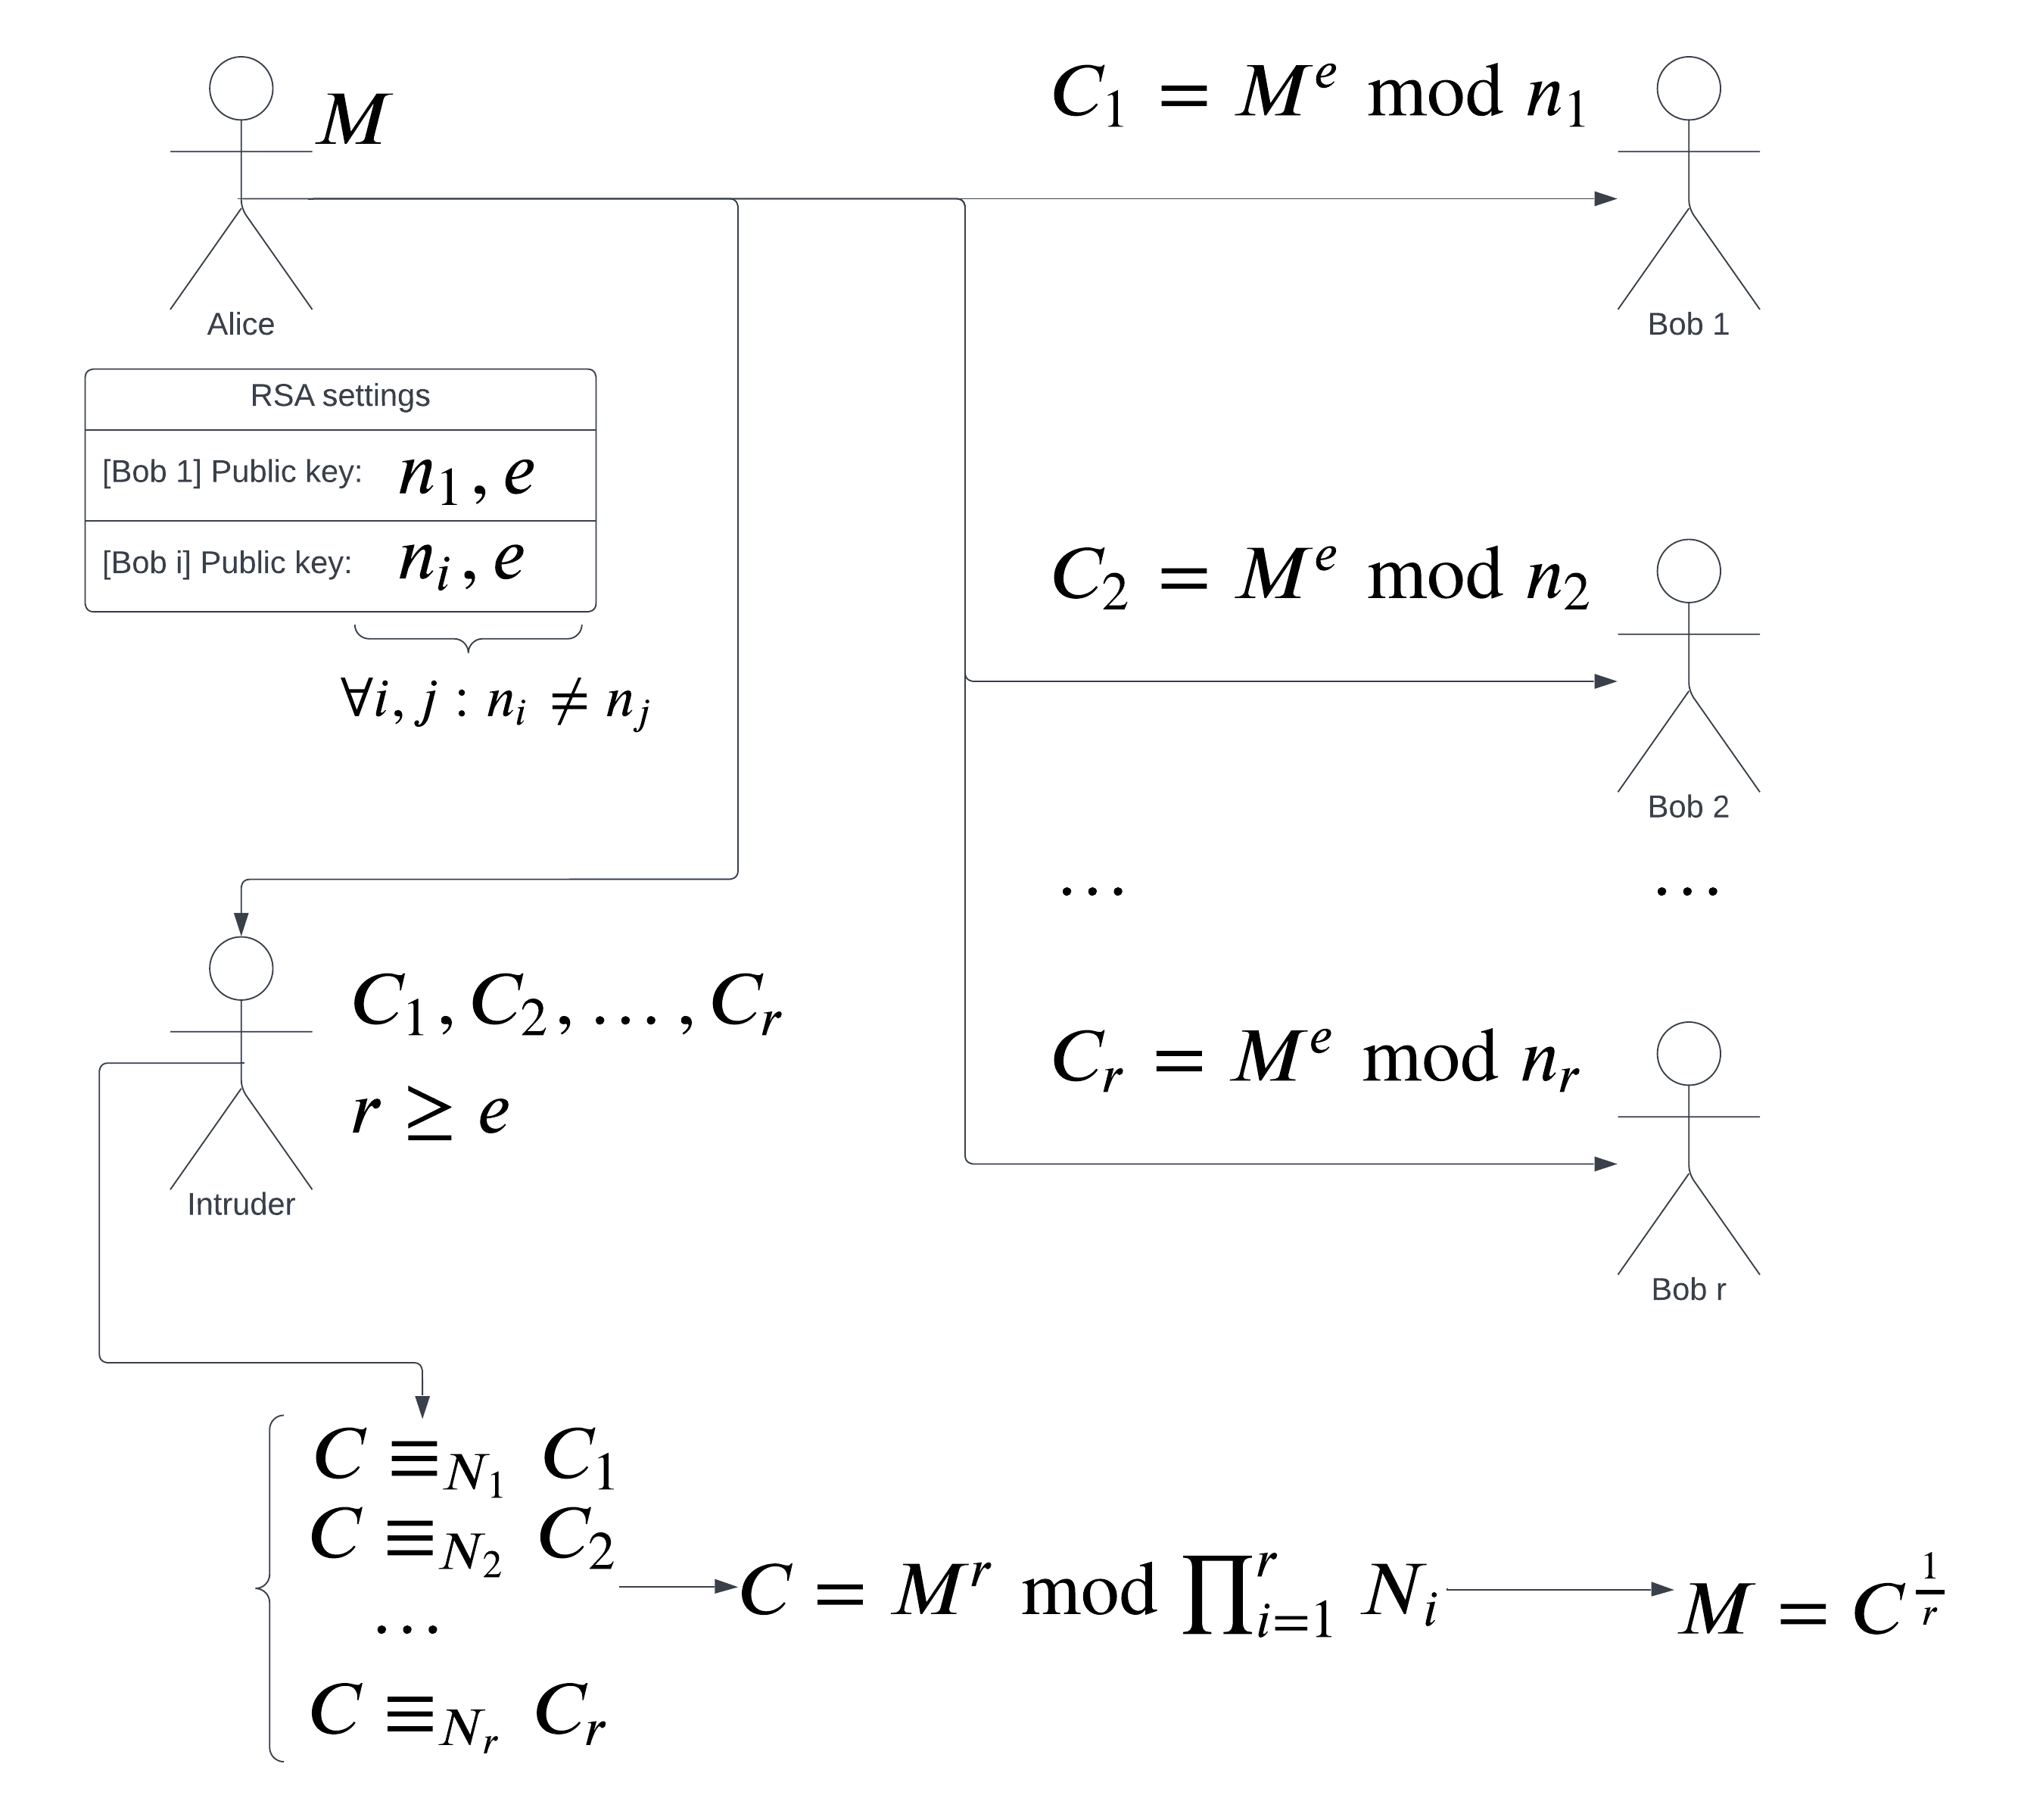
\includegraphics[width=\textwidth]{img/RSA_attack_broadcast.png}
    \caption{Another RSA attack on broadcast communication.}
\end{figure}

\subsection{Leaked $\varphi(n)$ RSA attack}
Consider an RSA cryptosystem, in which the $\varphi(n)$ value is somehow leaked. Remark that:
\begin{itemize}
    \item $n = p \cdot q$
    \item $\varphi(n) = (p - 1) \cdot (q - 1)$
\end{itemize}
Consider now what follows:
\begin{align*}
    \varphi(n) &= (p - 1) \cdot (q - 1) \\
    \varphi(n) &= (p \cdot q) - p - q + 1 \\
    \varphi(n) &= n - p - q + 1 \\
    p + q &= n - \varphi(n) + 1 \\
\end{align*}
This equation can be used to solve the following system:
\begin{align*}
    \begin{cases}
        p + q = n - \varphi(n) + 1\\
        n = p \cdot q
    \end{cases}& \rightarrow &
    \begin{cases}
        p + q = n - \varphi(n) + 1\\
        q = \frac{n}{q}
    \end{cases}\\
    \begin{cases}
        p + \frac{n}{q} = n - \varphi(n) + 1\\
        q = \frac{n}{q}
    \end{cases}& \rightarrow &
    \begin{cases}
        p^{2} + n = p(n - \varphi(n) + 1)\\
        q = \frac{n}{q}
    \end{cases}\\
    & \rightarrow &
    \begin{cases}
        p^{2} - p(n - \varphi(n) + 1) + n = 0\\
        q = \frac{n}{q}
    \end{cases}
\end{align*}

The solution to the first equation is trivial, since it's sufficent to apply the quadratic formula to retrieve the solutions for $p$; this can easily lead to the solution for $q$ as well.

\section{Attacks to Block Ciphers}
\subsection{Known plaintext attack to an Affine block cipher}
Consider the following cryptosystem:
\begin{align*}
    \Sigma = \mathbb{Z}_{N}
    \mathcal{M} = \mathcal{C} = \mathbb{Z}_{N}^{\mathcal{l}} \\
    K_{E} = (A, b), K_{D} = (A^{-1}, b)\\
    \mathcal{f}: \mathbb{Z}_{N}^{\mathcal{l}} &\rightarrow \mathbb{Z}_{N}^{\mathcal{l}} \\
    m &\rightarrow (A \cdot m + b) \bmod N \\
    \mathcal{f}^{-1}: \mathbb{Z}_{N}^{\mathcal{l}} &\rightarrow \mathbb{Z}_{N}^{\mathcal{l}} \\
    c &\rightarrow A^{-1}(c - b) \bmod N \\
\end{align*}
Where:
\begin{itemize}
    \item $N > 0 \in \mathbb{N}$;
    \item $\mathcal{l} \geq 1 \in \mathbb{Z} $;
    \item $A$ is an invertible $\mathcal{l} \times \mathcal{l}$ matrix, and $\forall 1 \leq i,j \leq \mathcal{l}: A_{i,j} \in \mathbb{Z}$.
    \item $b \in \mathbb{Z}_{N}^{\mathcal{l}}$
\end{itemize}
Note that:
\begin{itemize}
    \item When $\mathcal{l} = 1, $ you get the Caesar's method;
    \item When $A = I$\footnote{The identity matrix.} and $b \in \mathbb{Z}_{N}^{\mathcal{l}}$ you get the Vigenére's method.
\end{itemize}
The attacks is conducted as follows:
\begin{enumerate}
    \item The intruder generates $\mathcal{l} + 1$ plaintexts ($p_{0}, \dots, p_{\mathcal{l}}$);
    \item The intruder collects the corrispondent ciphertexts ($c_{0}, \dots, c_{\mathcal{l}}$); Consider that:
    \[c_{i} \equiv A \cdot p_{i} + b \bmod N\]
    \item Now, consider that:
    \[c_{i} - c_{0} \equiv A \cdot p_{i} + b - A \cdot p_{0} - b \bmod N\]
    \item Then we define two matrixes:
    \[C = (c_{1} - c_{0}, \dots, c_{\mathcal{l}} - c_{0}), P = (p_{1} - p_{0}, \dots, p_{\mathcal{l}} - p_{0})\]
    \item So, we have that, if $(det P, N) = 1 \implies P$ is invertible:
    \begin{align*}
        C &\equiv A \cdot P \bmod N\\
        \iff C \cdot P^{-1} &\equiv A \cdot P \cdot P^{-1} \bmod N \\
        A \equiv C \cdot P^{-1} \bmod N  &\land b \equiv c_{0} - A \cdot p_{0} \bmod N
    \end{align*}
\end{enumerate}

\begin{figure}[h]
    \centering
    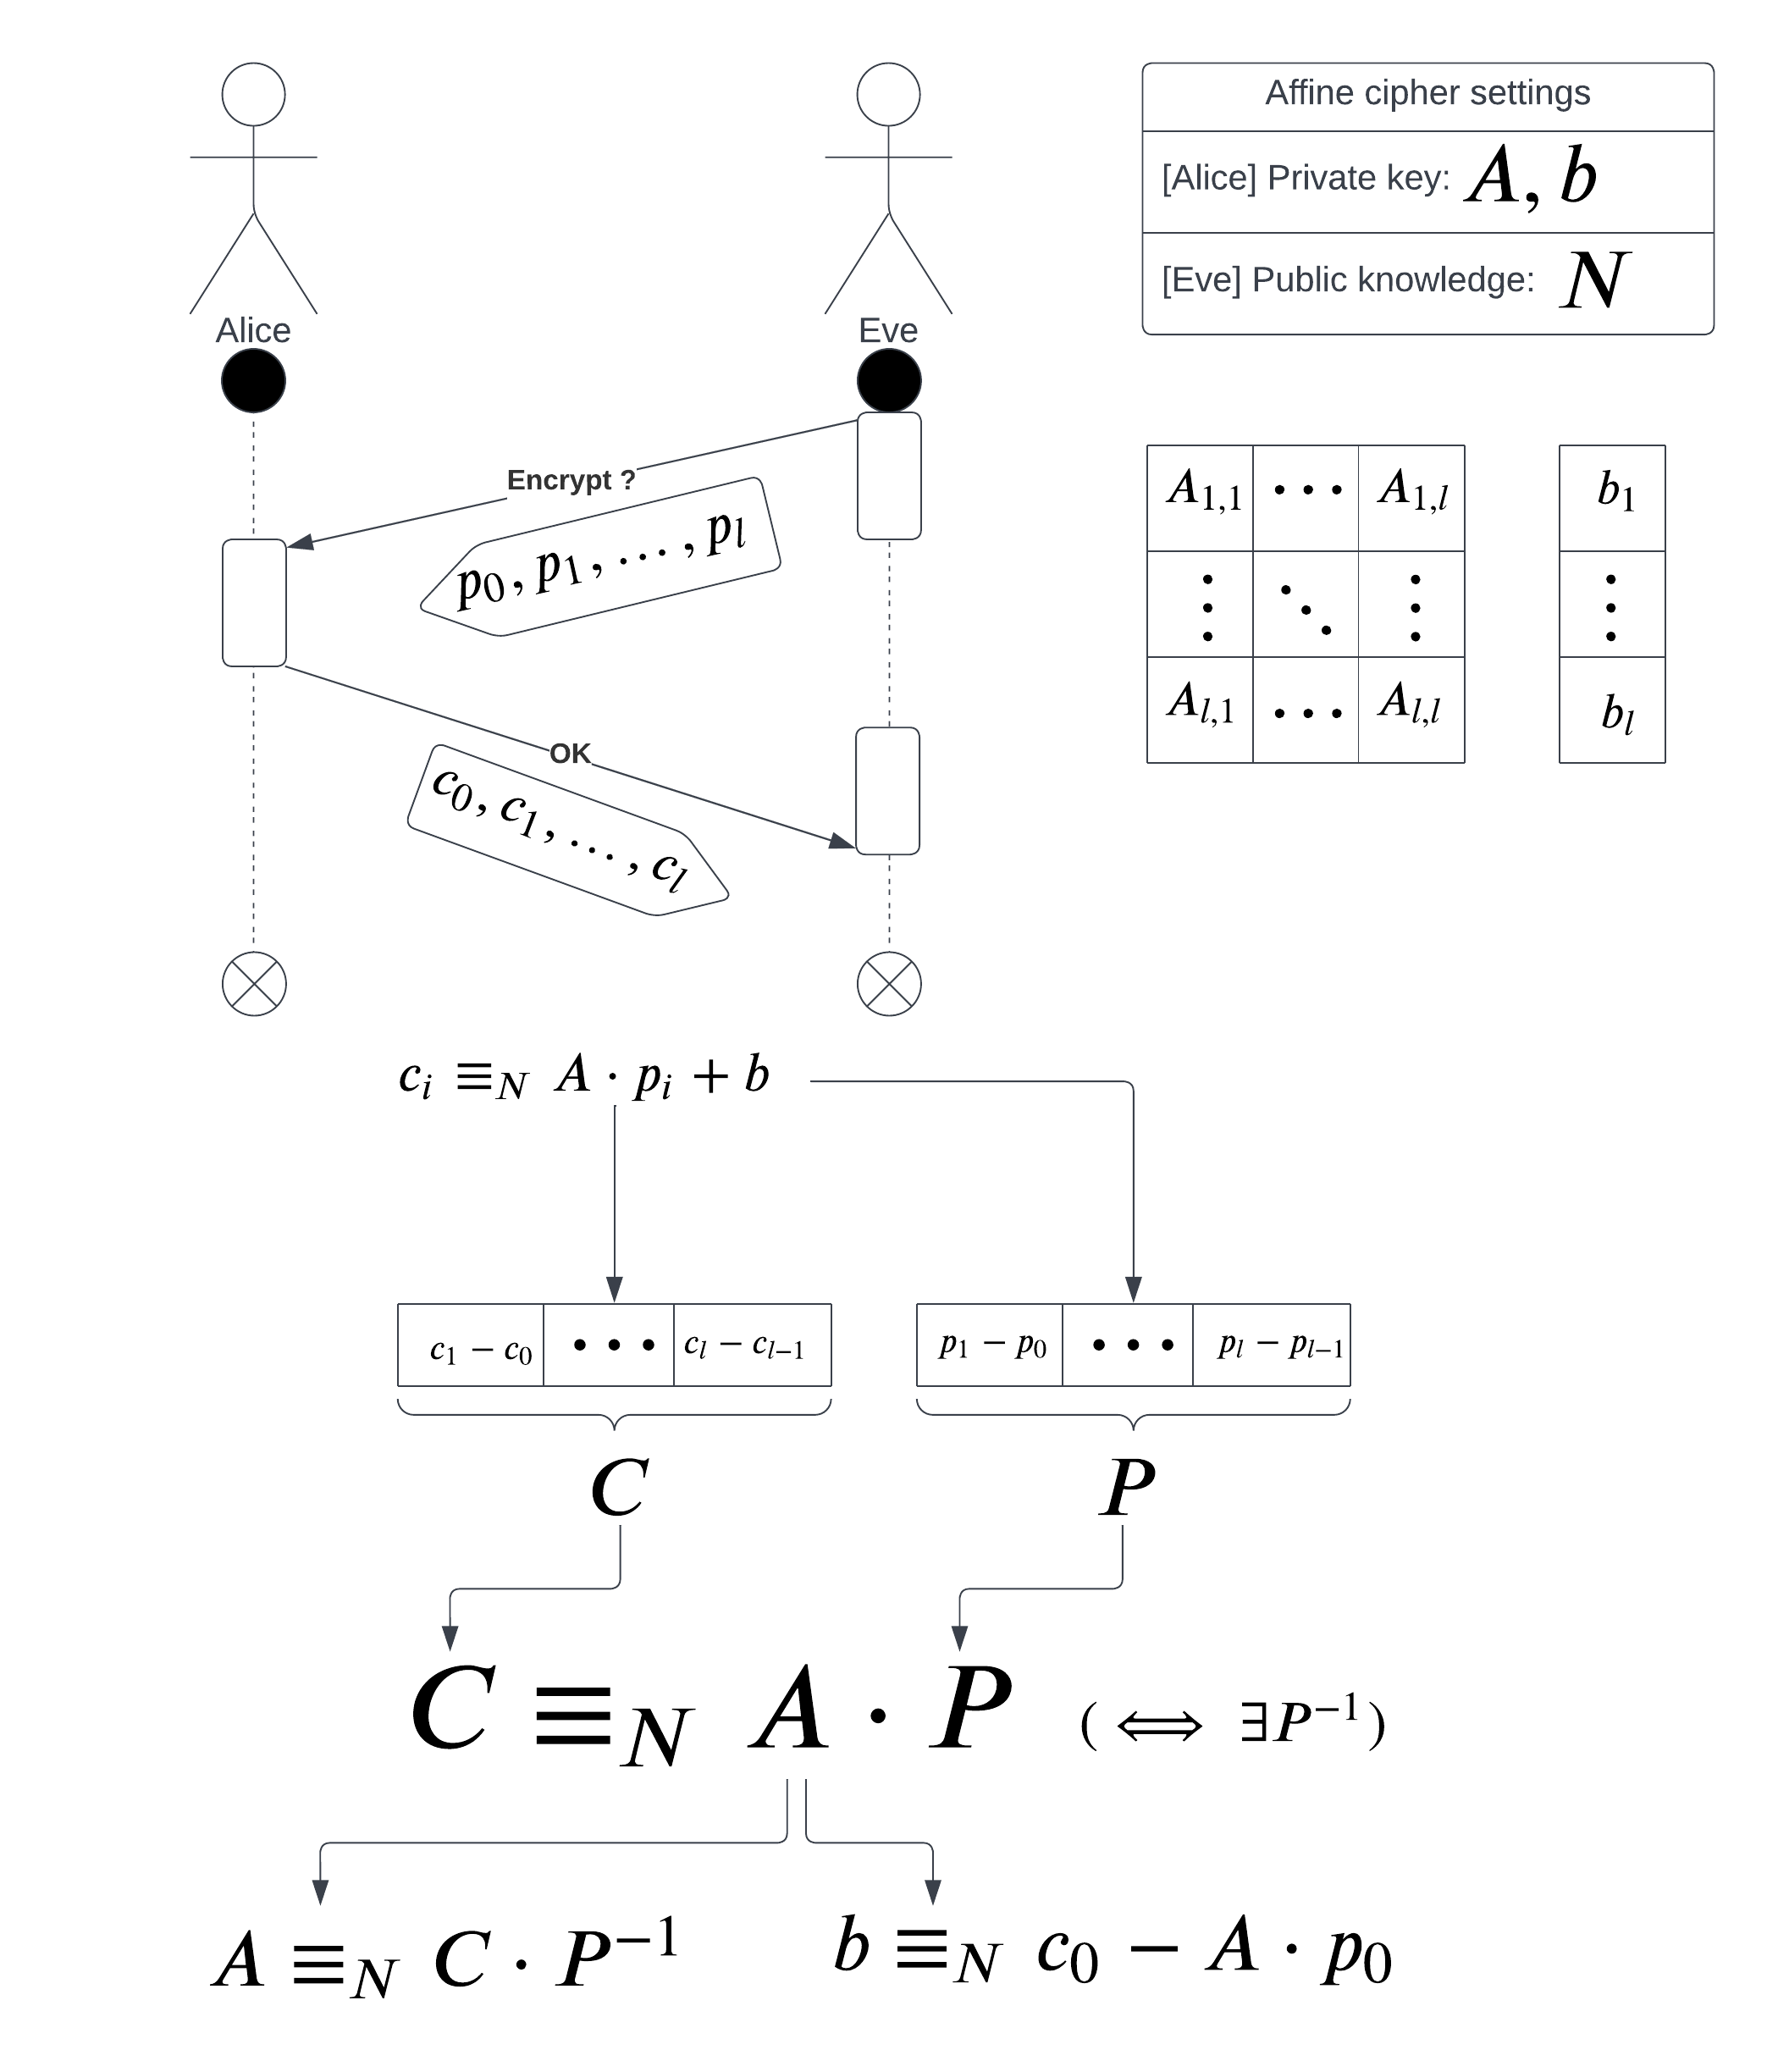
\includegraphics[width=\textwidth]{img/Affine_Block_Cipher_Known-plaintext_Attack.png}
    \caption{Known plaintext attack to an Affine block cipher.}
\end{figure}
